% Why each hypothesis exists: architectural fact -> consequence -> hypothesis.
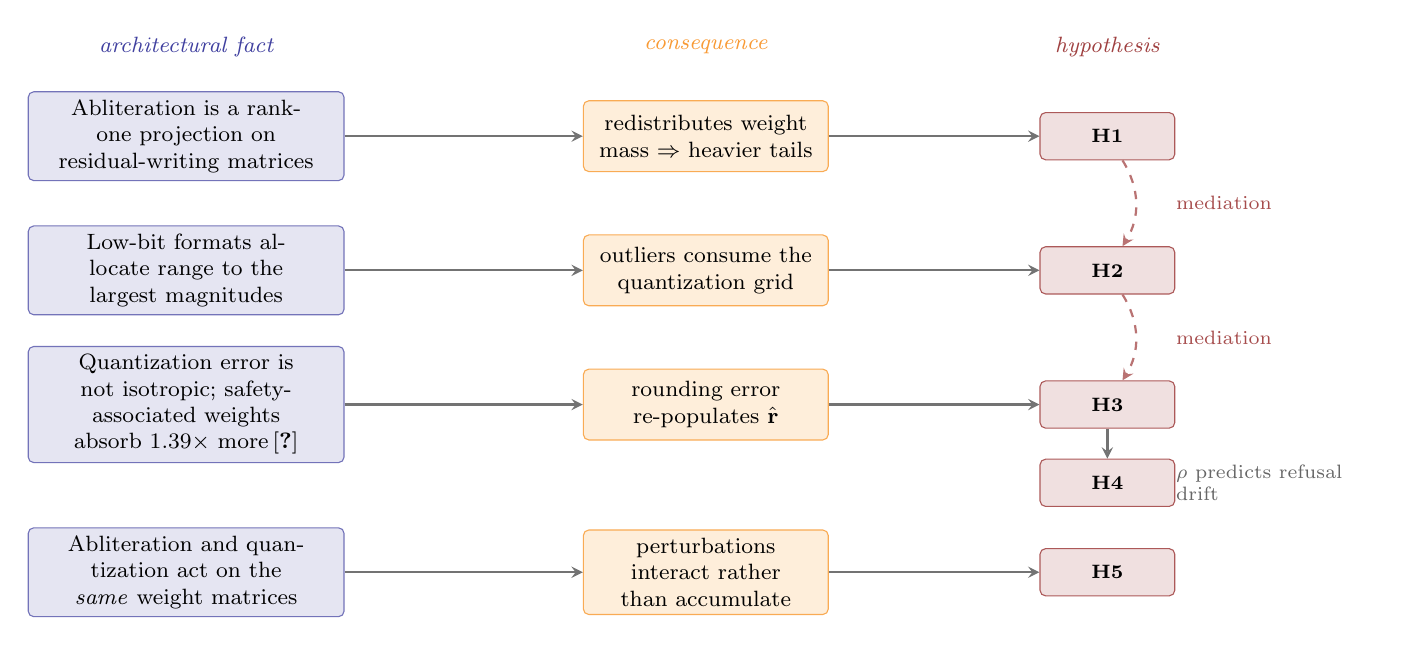
\begin{tikzpicture}[
  font=\footnotesize, x=1.5mm, y=1.42mm, >=stealth,
  fact/.style={draw=NavyBlue!55, fill=NavyBlue!10, rounded corners=2pt,
               text width=38mm, align=center, inner sep=3pt, minimum height=9mm},
  mech/.style={draw=BurntOrange!65, fill=BurntOrange!12, rounded corners=2pt,
               text width=29mm, align=center, inner sep=3pt, minimum height=9mm},
  hyp/.style={draw=Maroon!65, fill=Maroon!12, rounded corners=2pt,
              text width=15mm, align=center, inner sep=3pt, minimum height=6mm,
              font=\scriptsize\bfseries},
  ar/.style={->, black!55, thick},
]
% column headers
\node[font=\footnotesize\itshape, text=NavyBlue!75] at (0,25) {architectural fact};
\node[font=\footnotesize\itshape, text=BurntOrange!80] at (44,25) {consequence};
\node[font=\footnotesize\itshape, text=Maroon!75] at (78,25) {hypothesis};

\node[fact] (f1) at (0,17) {Abliteration is a rank-one projection on residual-writing matrices};
\node[fact] (f2) at (0,5) {Low-bit formats allocate range to the largest magnitudes};
\node[fact] (f3) at (0,-7) {Quantization error is not isotropic; safety-associated weights absorb $1.39\times$ more\,\cite{qualitynotproxy2026}};
\node[fact] (f4) at (0,-22) {Abliteration and quantization act on the \emph{same} weight matrices};

\node[mech] (m1) at (44,17) {redistributes weight mass $\Rightarrow$ heavier tails};
\node[mech] (m2) at (44,5) {outliers consume the quantization grid};
\node[mech] (m3) at (44,-7) {rounding error re-populates $\hat{\mathbf r}$};
\node[mech] (m4) at (44,-22) {perturbations interact rather than accumulate};

\node[hyp] (h1) at (78,17) {H1};
\node[hyp] (h2) at (78,5) {H2};
\node[hyp] (h3) at (78,-7) {H3};
\node[hyp] (h4) at (78,-14) {H4};
\node[hyp] (h5) at (78,-22) {H5};

\foreach \f/\m in {f1/m1, f2/m2, f3/m3, f4/m4} \draw[ar] (\f) -- (\m);
\draw[ar] (m1) -- (h1);
\draw[ar] (m2) -- (h2);
\draw[ar] (m3) -- (h3);
\draw[ar] (m4) -- (h5);
\draw[ar] (h3) -- (h4);

% the chain across hypotheses
\draw[ar, Maroon!55, dashed] (h1) to[bend left=32] (h2);
\draw[ar, Maroon!55, dashed] (h2) to[bend left=32] (h3);
\node[font=\scriptsize, text=Maroon!70, anchor=west] at (83,11) {mediation};
\node[font=\scriptsize, text=Maroon!70, anchor=west] at (83,-1) {mediation};
\node[font=\scriptsize, text=black!60, anchor=west, text width=26mm] at (83,-14)
  {$\rho$ predicts refusal drift};
\end{tikzpicture}
